\documentclass[11pt]{article}

% font things
\usepackage{amsmath}
\usepackage{MnSymbol} % math things
% serif: if MinionPro doesn't work, use mathptmx
\usepackage[lf, mathtabular, minionint]{MinionPro} % Minion
% \usepackage{mathptmx}   % times
% sans font: use roboto if MyriadPro doesn't work
% \usepackage{MyriadPro} 
\usepackage{roboto}     % sans 


% begin old preamble

% --- character encoding ---
% \usepackage[latin1]{inputenc}
% \usepackage[T1]{fontenc}


\usepackage[top=.8in, bottom=.8in, left=1in, right=1in]{geometry}

% --- old font ---
% \renewcommand{\rmdefault}{pplx}
% \usepackage[sc]{mathpazo}
% \usepackage[OT1, euler-hat-accent]{eulervm}
\usepackage[usenames, dvipsnames, svgnames]{xcolor}
\usepackage{enumitem}

% --- styling ---
\usepackage{titling}
\usepackage[small, compact]{titlesec}
\setitemize[0]{leftmargin=*}
\usepackage{multicol, multirow}
\usepackage{epsfig, subfigure, subfloat, graphicx}
\usepackage{anysize, indentfirst, setspace}
\usepackage{verbatim, rotating, xfrac}
\usepackage{gensymb}
\usepackage{caption, hanging}
\newcommand{\mc}[1]{\multicolumn{1}{c}{#1}}
%\parindent 0pt
%\setdefaultenum{a.}{i.}{A}{1}
%\setdefaultitem{}{\textperiodcentered}{}{}
\usepackage{booktabs}
\usepackage{dcolumn}
\usepackage{caption, hanging}
\usepackage{tikz}
\usetikzlibrary{shapes,arrows,backgrounds}
%\setdefaultenum{a.}{1)}{i.}{a.}
\parindent 0pt

\makeatletter
\newcommand{\distas}[1]{\mathbin{\overset{#1}{\kern\z@\sim}}}%
\newsavebox{\mybox}\newsavebox{\mysim}
\newcommand{\distras}[1]{%
  \savebox{\mybox}{\hbox{\kern3pt$\scriptstyle#1$\kern3pt}}%
  \savebox{\mysim}{\hbox{$\sim$}}%
  \mathbin{\overset{#1}{\kern\z@\resizebox{\wd\mybox}{\ht\mysim}{$\sim$}}}%
}
\makeatother




\title{\Large{\bf{\vspace{-100pt}Mathematics for Political Science \vspace{-15pt}}}}
\author{\large{Day 1: Introduction, Foundations, Pre-Calculus}}
\date{\vspace{-5pt}\large{Solutions \vspace{-10pt}}}
\begin{document}


\maketitle

\hrule




\begin{enumerate}

 \item \begin{enumerate}[nosep]
  \item Discrete, Discrete, Discrete (would accept continuous, especially if half-points were allowed), Dichotomous, Discrete, Discrete
  \item Categorical, Categorical, Ratio, Categorical, Ordinal, Categorical
 \end{enumerate}


\item
\begin{itemize}
\item $f(g(x)) = 49 - 28x^3 + 4x^6$
\item $g(f(x)) = 2(3-x)^6-4$
\end{itemize}

\begin{small}
\begin{center}
\begin{tabular}{c|c|c|c|c}
x & $f(x) = (3-x)^2$  & $g(x) = 2x^3 - 4$   & $f(g(x))$  & $g(f(x))$\\ \hline
2 &   1               &       12            &   81       &   -2      \\
4 &  1                &      124            &   14641    &   -2      \\
5 &      4            &      246            &   59049    &   124     \\
1 &      4            &     -2              &  25        &   124     \\
0 &       9           &     -4              &   49       &    1454   \\
1 &      4            &      -2             &    25      &   124     \\
\end{tabular}
\end{center}
\end{small}


\item 
\begin{enumerate}
\item $g(x) = 8x-2, f(x) = 4x^3$
\item $g(x)=3x-2, f(x) = 1/x$
\end{enumerate}


\item The open interval does not include the endpoint.  Since the interval is limited by (but does not include) 1, it would be possible to get infinitely close to (but never reach) that point, and any number less than 1 has another point greater than that but less than 1.


\item 
\begin{enumerate}
\item 
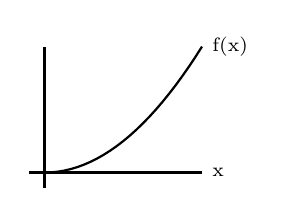
\begin{tikzpicture}[scale=.2]
\draw[thick] (-1,0) -- (10,0) node[right] {\scriptsize{x}};
\draw[thick] (0,-1) -- (0,8);
\draw[thick, domain=0:10] plot (\x,\x^2/12.5)node[right] {\scriptsize{f(x)}};
\end{tikzpicture}


\item 
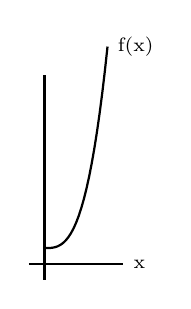
\begin{tikzpicture}[scale=.2]
\draw[thick] (-1,0) -- (5,0) node[right] {\scriptsize{x}};
\draw[thick] (0,-1) -- (0,12);
\draw[thick, domain=0:4] plot (\x,1 + .2*\x^3) node[right] {\scriptsize{f(x)}};
\end{tikzpicture}


\item 
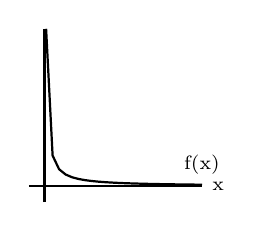
\begin{tikzpicture}[scale=.2]
\draw[thick] (-1,0) -- (10,0) node[right] {\scriptsize{x}};
\draw[thick] (0,-1) -- (0,10);
\draw[thick, domain=.1:10] plot (\x,1/\x)node[above] {\scriptsize{f(x)}};
\end{tikzpicture}


\item
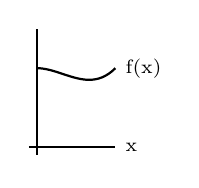
\begin{tikzpicture}[scale=1]
\draw[thick] (-.1,0) -- (1,0) node[right] {\scriptsize{x}};
\draw[thick] (0,-.1) -- (0,1.5);
\draw[thick, domain=0:1] plot (\x,1 - \x^2 + \x^3)node[right] {\scriptsize{f(x)}};
\end{tikzpicture}


\item 
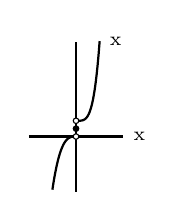
\begin{tikzpicture}[scale=.2]
\draw[thick] (-3,0) -- (3,0) node[right] {\scriptsize{x}};
\draw[thick] (0,-3.5) -- (0,6);
\draw[thick, domain=-1.5:-.001] plot (\x,\x^3);
\filldraw[black] (0,.5) circle (5pt);
\draw[thick, domain=.001:1.5] plot (\x,\x^4 + 1) node[right] {\scriptsize{x}};
\draw[black, fill=white] (0,0) circle (5pt);
\draw[black, fill=white] (0,1) circle (5pt);
\end{tikzpicture}
\end{enumerate}



\item Approximately linear growth: $p \approx 282,200,000 + 2,800,000*y$ (if we assume that $y = 0$ is the year 2,000)




\item ConCAVE looks like the entrance to a cave, conVex looks like a V.



\item 
\begin{enumerate}
\item monotonic
\item non-monotonic
\item non-monotonic
\end{enumerate}


\item 
\begin{enumerate}
\item $39/2$
\item $288$
\end{enumerate}


%\clearpage

\item 
\begin{tabular}{p{3cm}p{3cm}p{3cm}}
a. $-x^8y^4$            &  b. $9$                              & c. $8a^6$                     \rule{0cm}{1cm}\\
d. $x$                  &  e. $y^3 + y^4 + y^5$                & f. $\frac{10a}{77b}$          \rule{0cm}{1cm}\\
\rule{0cm}{1cm}\\ 
\end{tabular}



\item 
\begin{enumerate}
\item $a^2$
\item $3pq^2 + 6p^2 q + 3p^3 - pq + x(4q^2 + 16pq +16p^2)$
\end{enumerate}


\item 
\begin{enumerate}
\item B wins 29,000 to 28,000
\item \$265,625 more, for a total of \$1,265,625
\end{enumerate}


\item $56,000$






\item 
\begin{enumerate}
\item $x = \frac{1}{3}$
\item $x = \frac{3}{4}$
\end{enumerate}


\item 
\begin{enumerate}
\item $\alpha = \beta + 4\theta$
\item $\alpha = \frac{4}{(x + y - x^2 - y^2)}$
\end{enumerate}


\item 
\begin{enumerate}
\item $x > -18$
\item $t < 6$
\item $y \leq \frac{29}{22}$
\end{enumerate}


\item 
\begin{enumerate}
\item $x = 2$ or $x=-7$
\item $x=4$
\item $x=2$ or $x=-5$
\end{enumerate}


\item 
\begin{enumerate}
\item $x=\frac{1}{9}$ or $x=-1.5$
\item $x= -\frac{2}{7}$ or $x=\frac{4}{5}$
\end{enumerate}


\item 
\begin{enumerate}
\item $a=0$, $b=2$
\item $a=5$, $b=5$
\end{enumerate}



\item 
\begin{enumerate}
\item $c=7$, $d=-2$
\item $c=-3$, $d=4$
\end{enumerate}


\item $x=4\alpha + 2$, $y=2\alpha + 1$


\item $q=1$, $r=-1$, $s=3$


\item 
\begin{enumerate}
\item $25$
\item $22$
\end{enumerate}




\item Odd powers are identical to the matrix given; even powers are the identity matrix.


\item 
\[
\left[\begin{array}{cc}
a & b \\
c & d \\
\end{array}\right]
+
\left[\begin{array}{cc}
0 & 0 \\
0 & 0 \\
\end{array}\right]
=
\left[\begin{array}{cc}
a+0 & b+0 \\
c+0 & d+0 \\
\end{array}\right]
=
\left[\begin{array}{cc}
a & b \\
c & d \\
\end{array}\right]
\]

\[
\left[\begin{array}{cc}
a & b \\
c & d \\
\end{array}\right]
\left[\begin{array}{cc}
1 & 0 \\
0 & 1 \\
\end{array}\right]
=
\left[\begin{array}{cc}
a*1 + b*0 & a*0 + b*1 \\
c*1 + d*0 & c*0 + d*1 \\
\end{array}\right]
=
\left[\begin{array}{cc}
a & b \\
c & d \\
\end{array}\right]
\]


\item 
\begin{enumerate}
\item $\left[\begin{array}{cc}
56 & 70 \\
\end{array}\right]$
% [56  70]
\item $
\left[\begin{array}{c}
ap + bq + cr \\
dp + eq + fr \\
gp + hq + ir \\
\end{array}\right]$
\item The inner dimensions do not conform, so these matrices cannot be multiplied in this order.
\end{enumerate}




\item Multiply the matrices below to show that order matters for matrix multiplication: \\

\begin{enumerate}
\item $\left[\begin{array}{c}
17 \\
\end{array}\right]
~~~\textrm{or}~~~
\left[\begin{array}{ccc}
12 & 21 & 3 \\
0  & 0  & 0 \\
20 & 35 & 5 \\
\end{array}\right]$
\item $\left[\begin{array}{ccc}
44 & 64 & 36 \\
15 & 36 & 21 \\
20 & 22 & 12 \\
\end{array}\right]
~~~\textrm{or}~~~
\left[\begin{array}{cc}
48 & 114 \\
15 & 44 \\
\end{array}\right]$
\end{enumerate}







\end{enumerate}




\vfill
\begin{center}
\small{Thanks to Dave Ohls, Brad Jones, and Sarah Bouchat for past years' materials}
\end{center}

\end{document} 